\subsection{Retours d'expérience de précédents projets}
\label{subsec:retour_exp}

Le projet SP-02 bénéficie d’un retour d’expérience direct issu de 13 projets antérieurs auxquels les membres actuels de l’équipe
ont participé. Ce capital de compétences accumulé au fil des campagnes précédentes représente un atout majeur pour la maîtrise
technique du développement.\\

Au-delà de ce noyau d’expérience directe, le projet s’appuie sur l’héritage de l’association AéroIPSA, créée en 1992. Depuis sa
fondation, l’association a participé à 21 campagnes de lancement et présenté plus de 90 projets. Ces trente années d’activité ont
permis de constituer un corpus méthodologique et technique considérable, transmis entre promotions à travers les archives
internes, les rapports de vol, les plans mécaniques et les schémas électroniques documentant chaque réalisation.\cite{AeroIPSA}\\

Parmi les projets récents ayant eu l’influence la plus marquante sur le développement de SP-02, on distingue :\\

\begin{itemize}
    \item \textbf{Arcturus (2023-2024)} – \gls{Minif} dirigée par Lucas Pichon.\newline
    Arcturus a appliqué les méthodes de fabrication composites déjà éprouvées au sein d’AéroIPSA. La fusée reposait sur une
    peau porteuse en fibre de verre, des ailerons collés directement sur la paroi externe du fuselage et un système d’éjection
    du parachute par trappe latérale commandée électroniquement par minuterie. Ces techniques seront reprises pour la conception
    du second étage de SP-02, où les contraintes mécaniques et dimensionnelles sont similaires. (\cite{Arcturus})

\begin{figure}[h]
    \centering
    
\includegraphics[width=0.55\textwidth]{figures/arcturus.png}
    \caption{Minif Arcturus}
    \label{fig:arcturus}
\end{figure}

    \item \textbf{SP-01 (2023-2024)} – \gls{Fusex} dirigée par Malo Amaranti et Mathieu Coquelle-Grandsimon.\newline
    SP-01 reprenait la même logique structurelle et a permis de les perfectionner – peau porteuse composite, ailerons en fibre
    de verre, trappe latérale d’éjection du parachute, coiffe en composite – mais selon une approche différente pour le bloc
    propulseur. Les ailerons étaient insérés dans la fusée par des fentes et collés sur un tube propulseur interne, assurant une
    liaison rigide entre propulsion et structure. L’ensemble était collé à la résine époxy, garantissant la tenue à la poussée.
    Le projet introduisait également un rétreint à la base du fuselage, améliorant le profil aérodynamique, procédé directement
    réutilisé pour le premier étage de SP-02. Les essais et mesures embarquées ont validé le comportement mécanique de la
    structure et la fiabilité du système d’ouverture commandé, renforçant la base expérimentale du développement de SP-02.
    (\cite{SP01})

\begin{figure}[h]
    \centering
    
\includegraphics[width=0.8\textwidth]{figures/sp01_2.png}
    \caption{Fusée SP-01}
    \label{fig:sp01}
\end{figure}

\newpage

    \item \textbf{Unknown (2023-2024)} – module électronique embarqué développé par Vincent Fauquembergue.\newline
    Unknown, ayant volé sur SP-01, avait pour objectif la localisation des fusées et la collecte de données GNSS, barométriques
    et inertielles. Construit autour d’un STM32F411, il combinait télémesure LoRa, capteurs BMI088, BMP380, GPS SAM-M10Q et
    mémoire flash 16 Mo. Le vol a validé la chaîne de communication et la robustesse de l’intégration, établissant les bases
    matérielles et logicielles des futurs systèmes avioniques d’AéroIPSA. (\footnote{Le rapport de projet d'Unknown se trouve en
    annexe du rapport de projet d'SP-01\cite{SP01}})

\begin{figure}[h]
    \centering
    \begin{subfigure}{0.45\textwidth}
        \centering
        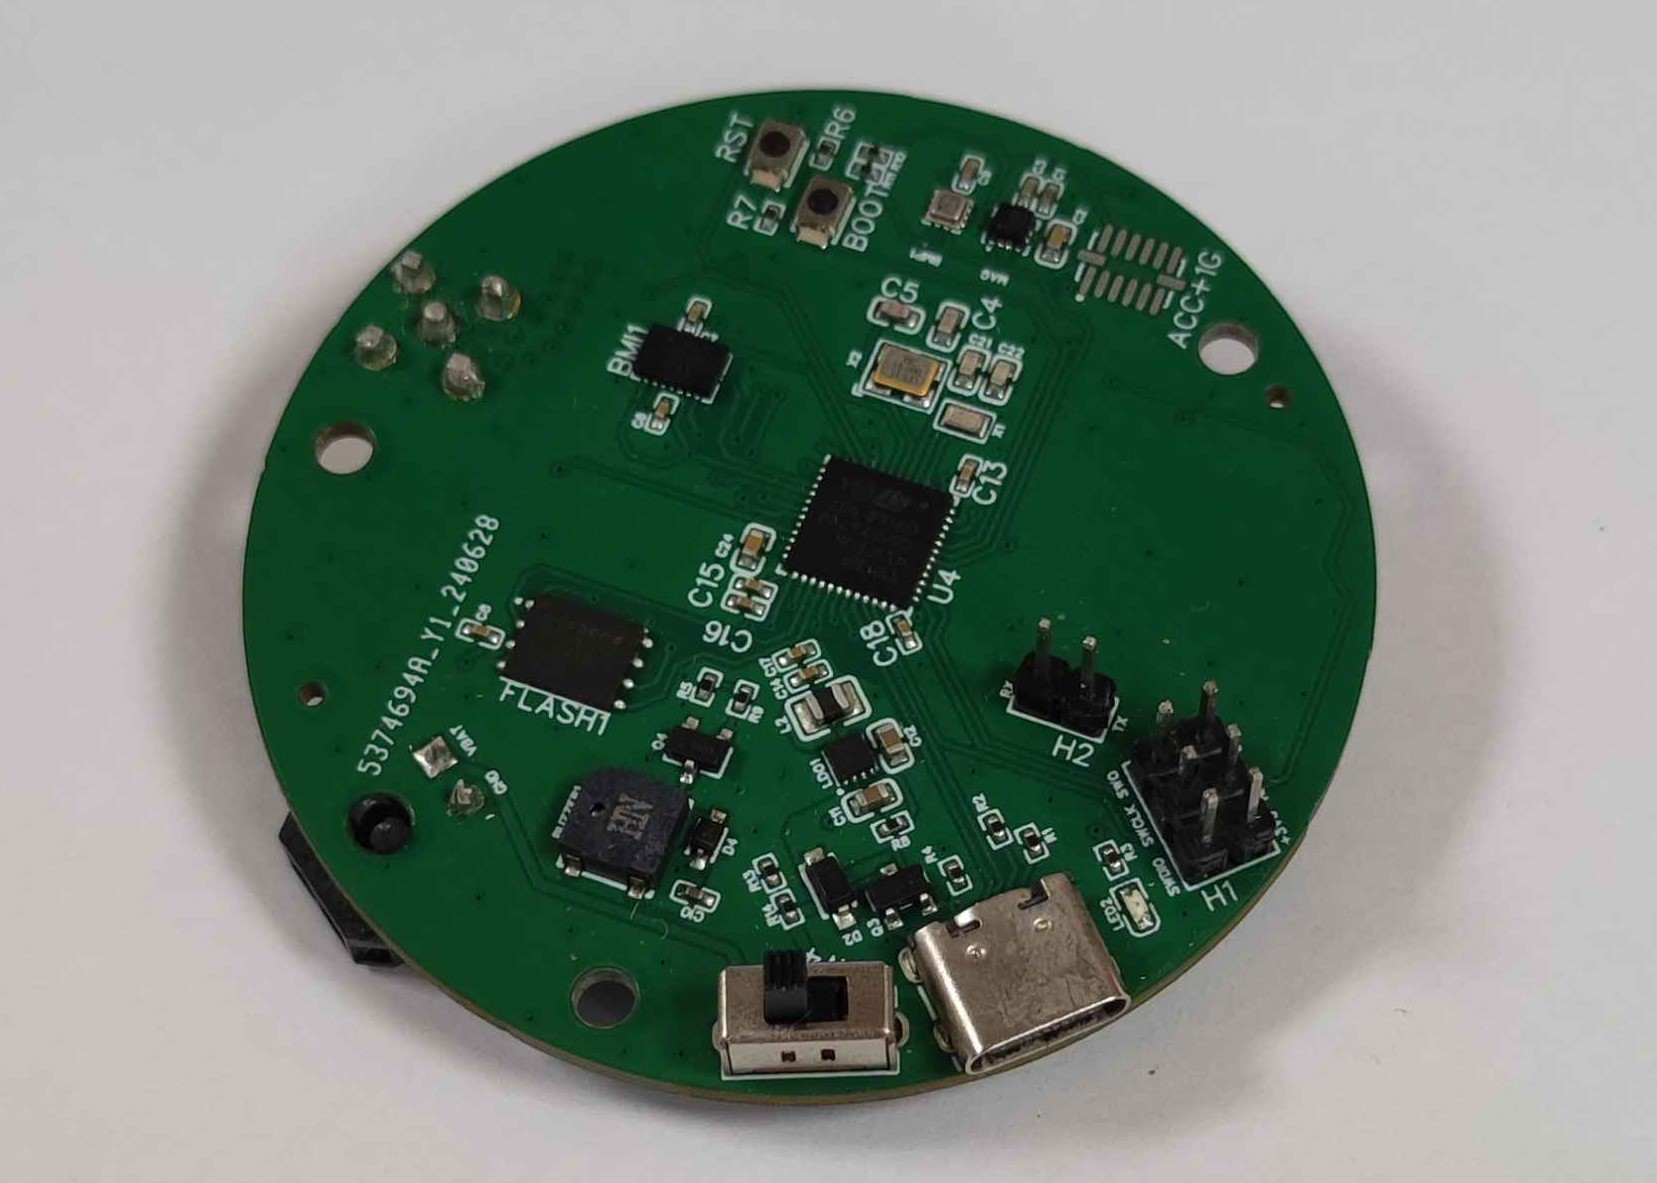
\includegraphics[width=0.8\textwidth]{figures/unknown1.jpg}
        \caption{face arrière}
        \label{fig:unknown1}
    \end{subfigure}
    \begin{subfigure}{0.45\textwidth}
        \centering
        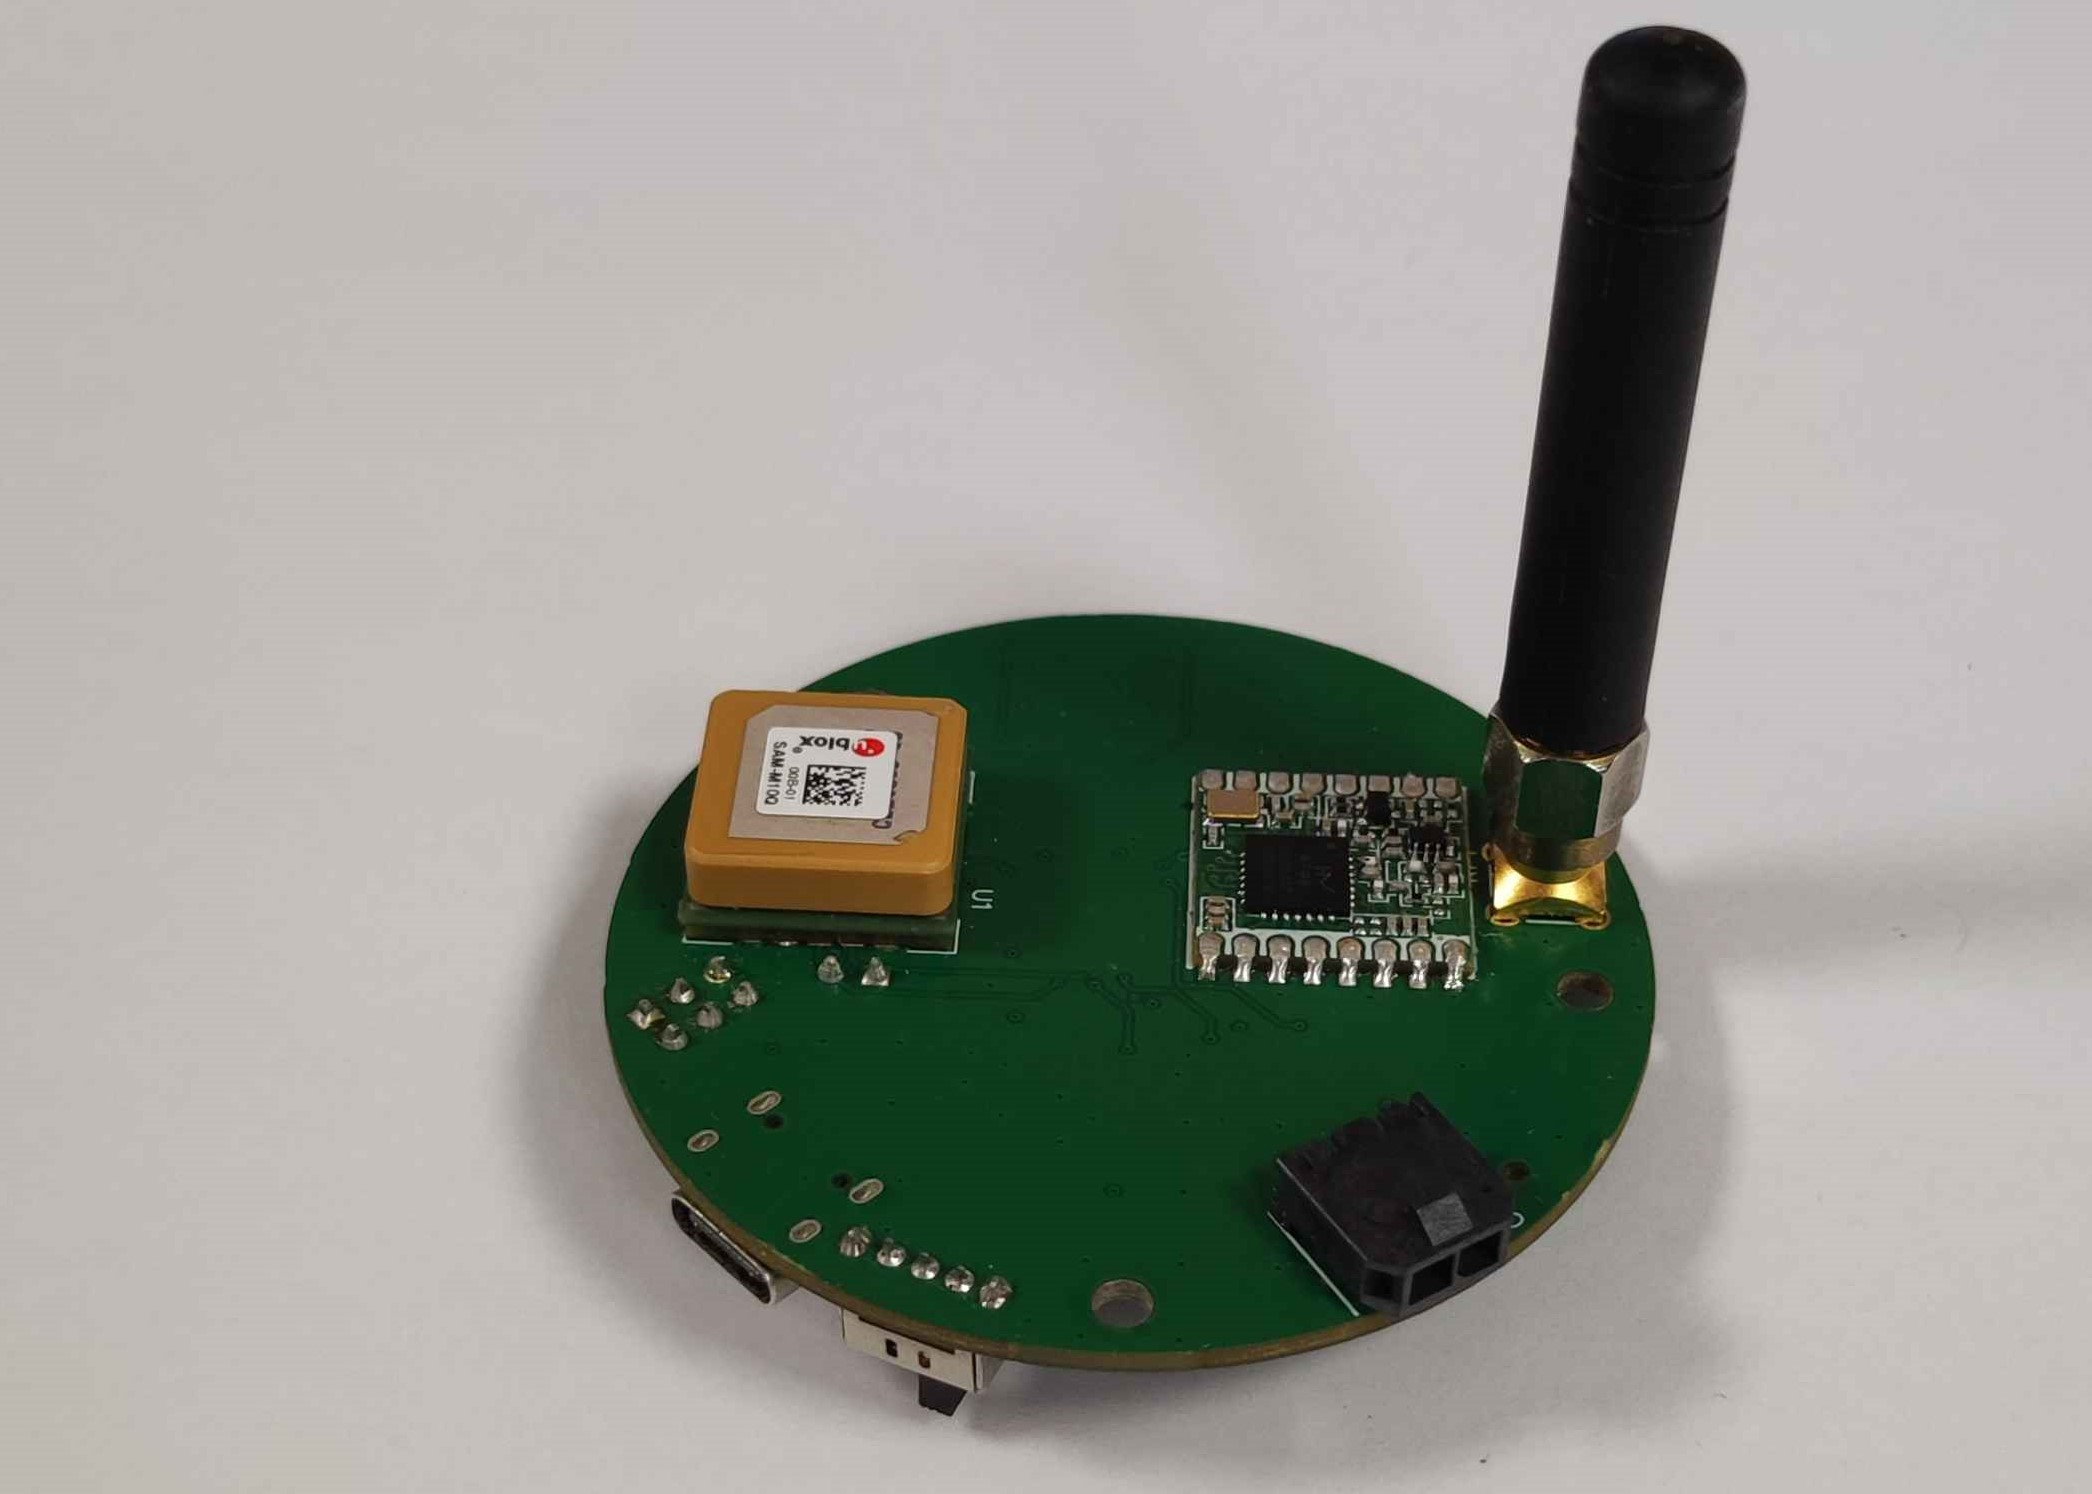
\includegraphics[width=0.8\textwidth]{figures/unknown2.jpg}
        \caption{face avant}
        \label{fig:unknown2}
    \end{subfigure}
    \caption{Module électronique Unknown}
\end{figure}

    \item \textbf{\gls{APEX} (2024-2025)} – évolution directe d’Unknown, dirigée par Malo Amaranti et Alexis Paillard.\newline
    Le projet a donné naissance à un module avionique intégré reposant sur le STM32F411RETx, la mémoire W25Q512 (64 Mo), le
    module LoRa RFM95W, et un ensemble complet de capteurs (BMI088, ADXL375, LSM303AGR, BMP380, SAM-M10Q). \gls{APEX} a été testé
    sur plusieurs fusées de la campagne 2025: MROM, Prisma et Horizon, et a démontré la fiabilité mécanique et l’autonomie
    énergétique du module, tout en identifiant des axes d’amélioration logicielle (synchronisation, filtrage et gestion de la
    mémoire). Le système avionique de SP-02 utilisera directement cette architecture matérielle et son logicielle sera
    directement issue des expériences passé des projets Unknown et \gls{APEX}. (\cite{APEX})

\begin{figure}[h]
    \centering
    \begin{subfigure}{0.45\textwidth}
        \centering
        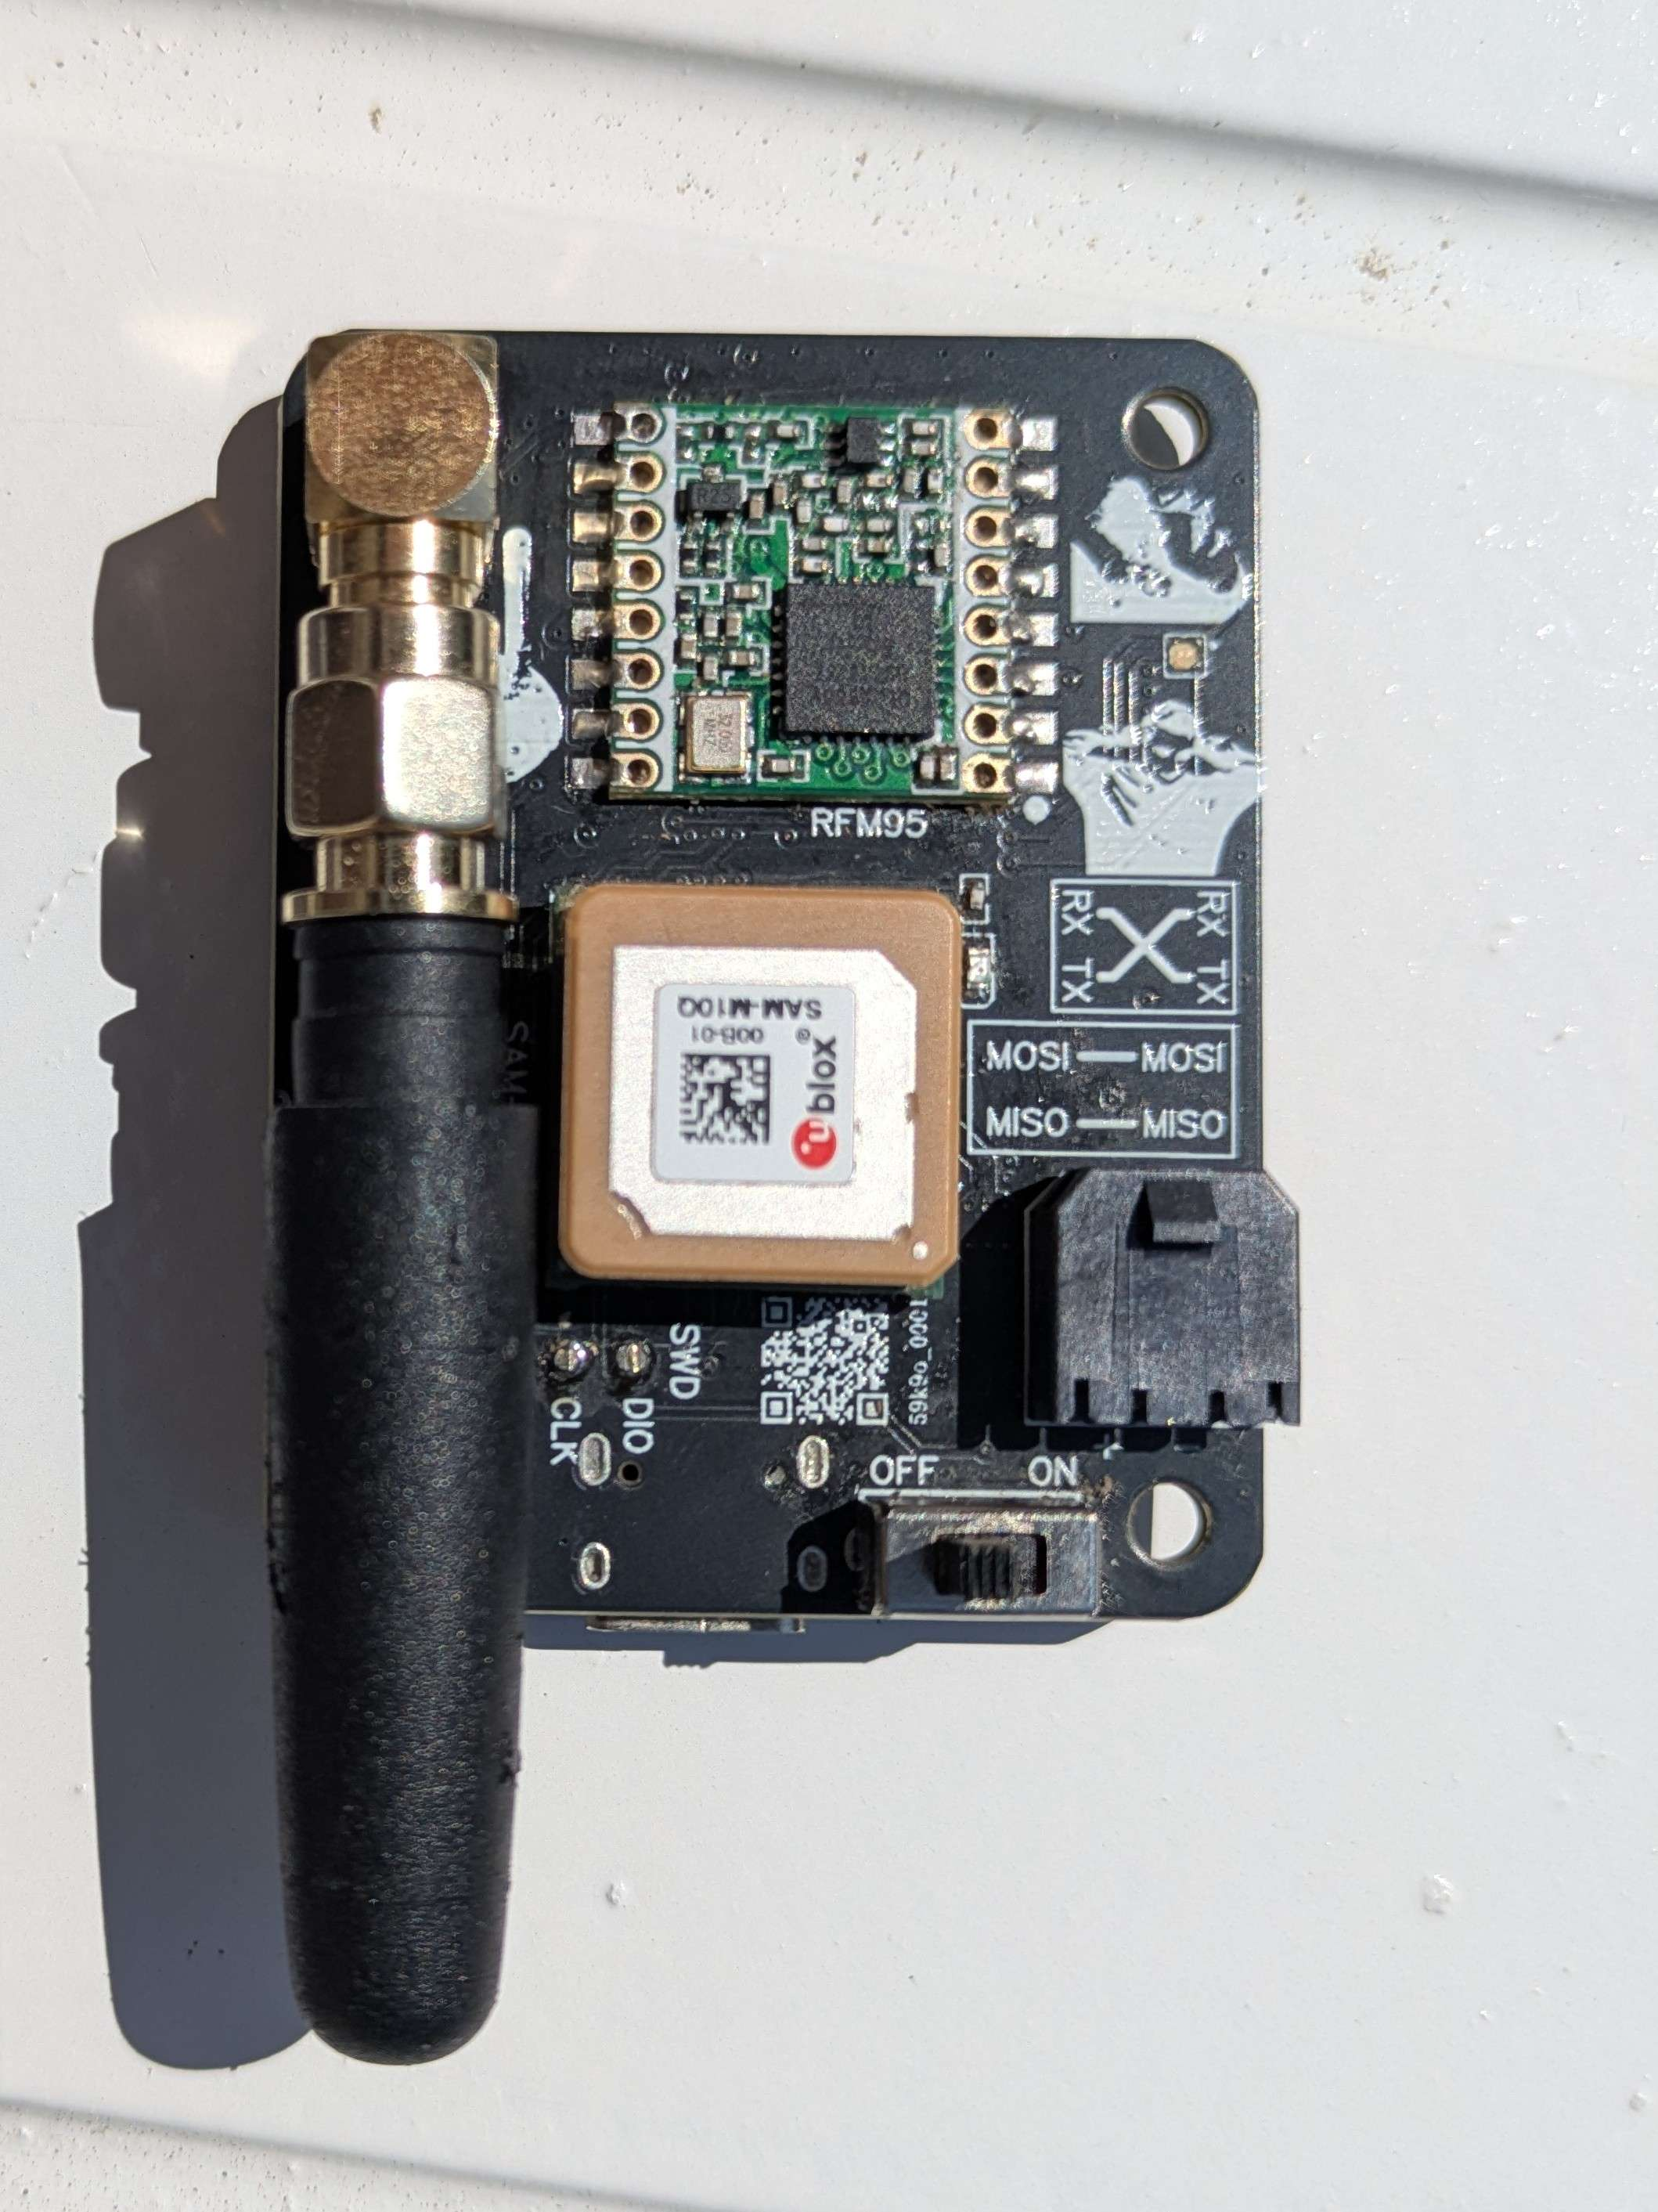
\includegraphics[width=0.7\textwidth]{figures/APEX_BACK.jpg}
        \caption{face arrière}
        \label{fig:apex_back}
    \end{subfigure}
    \begin{subfigure}{0.45\textwidth}
        \centering
        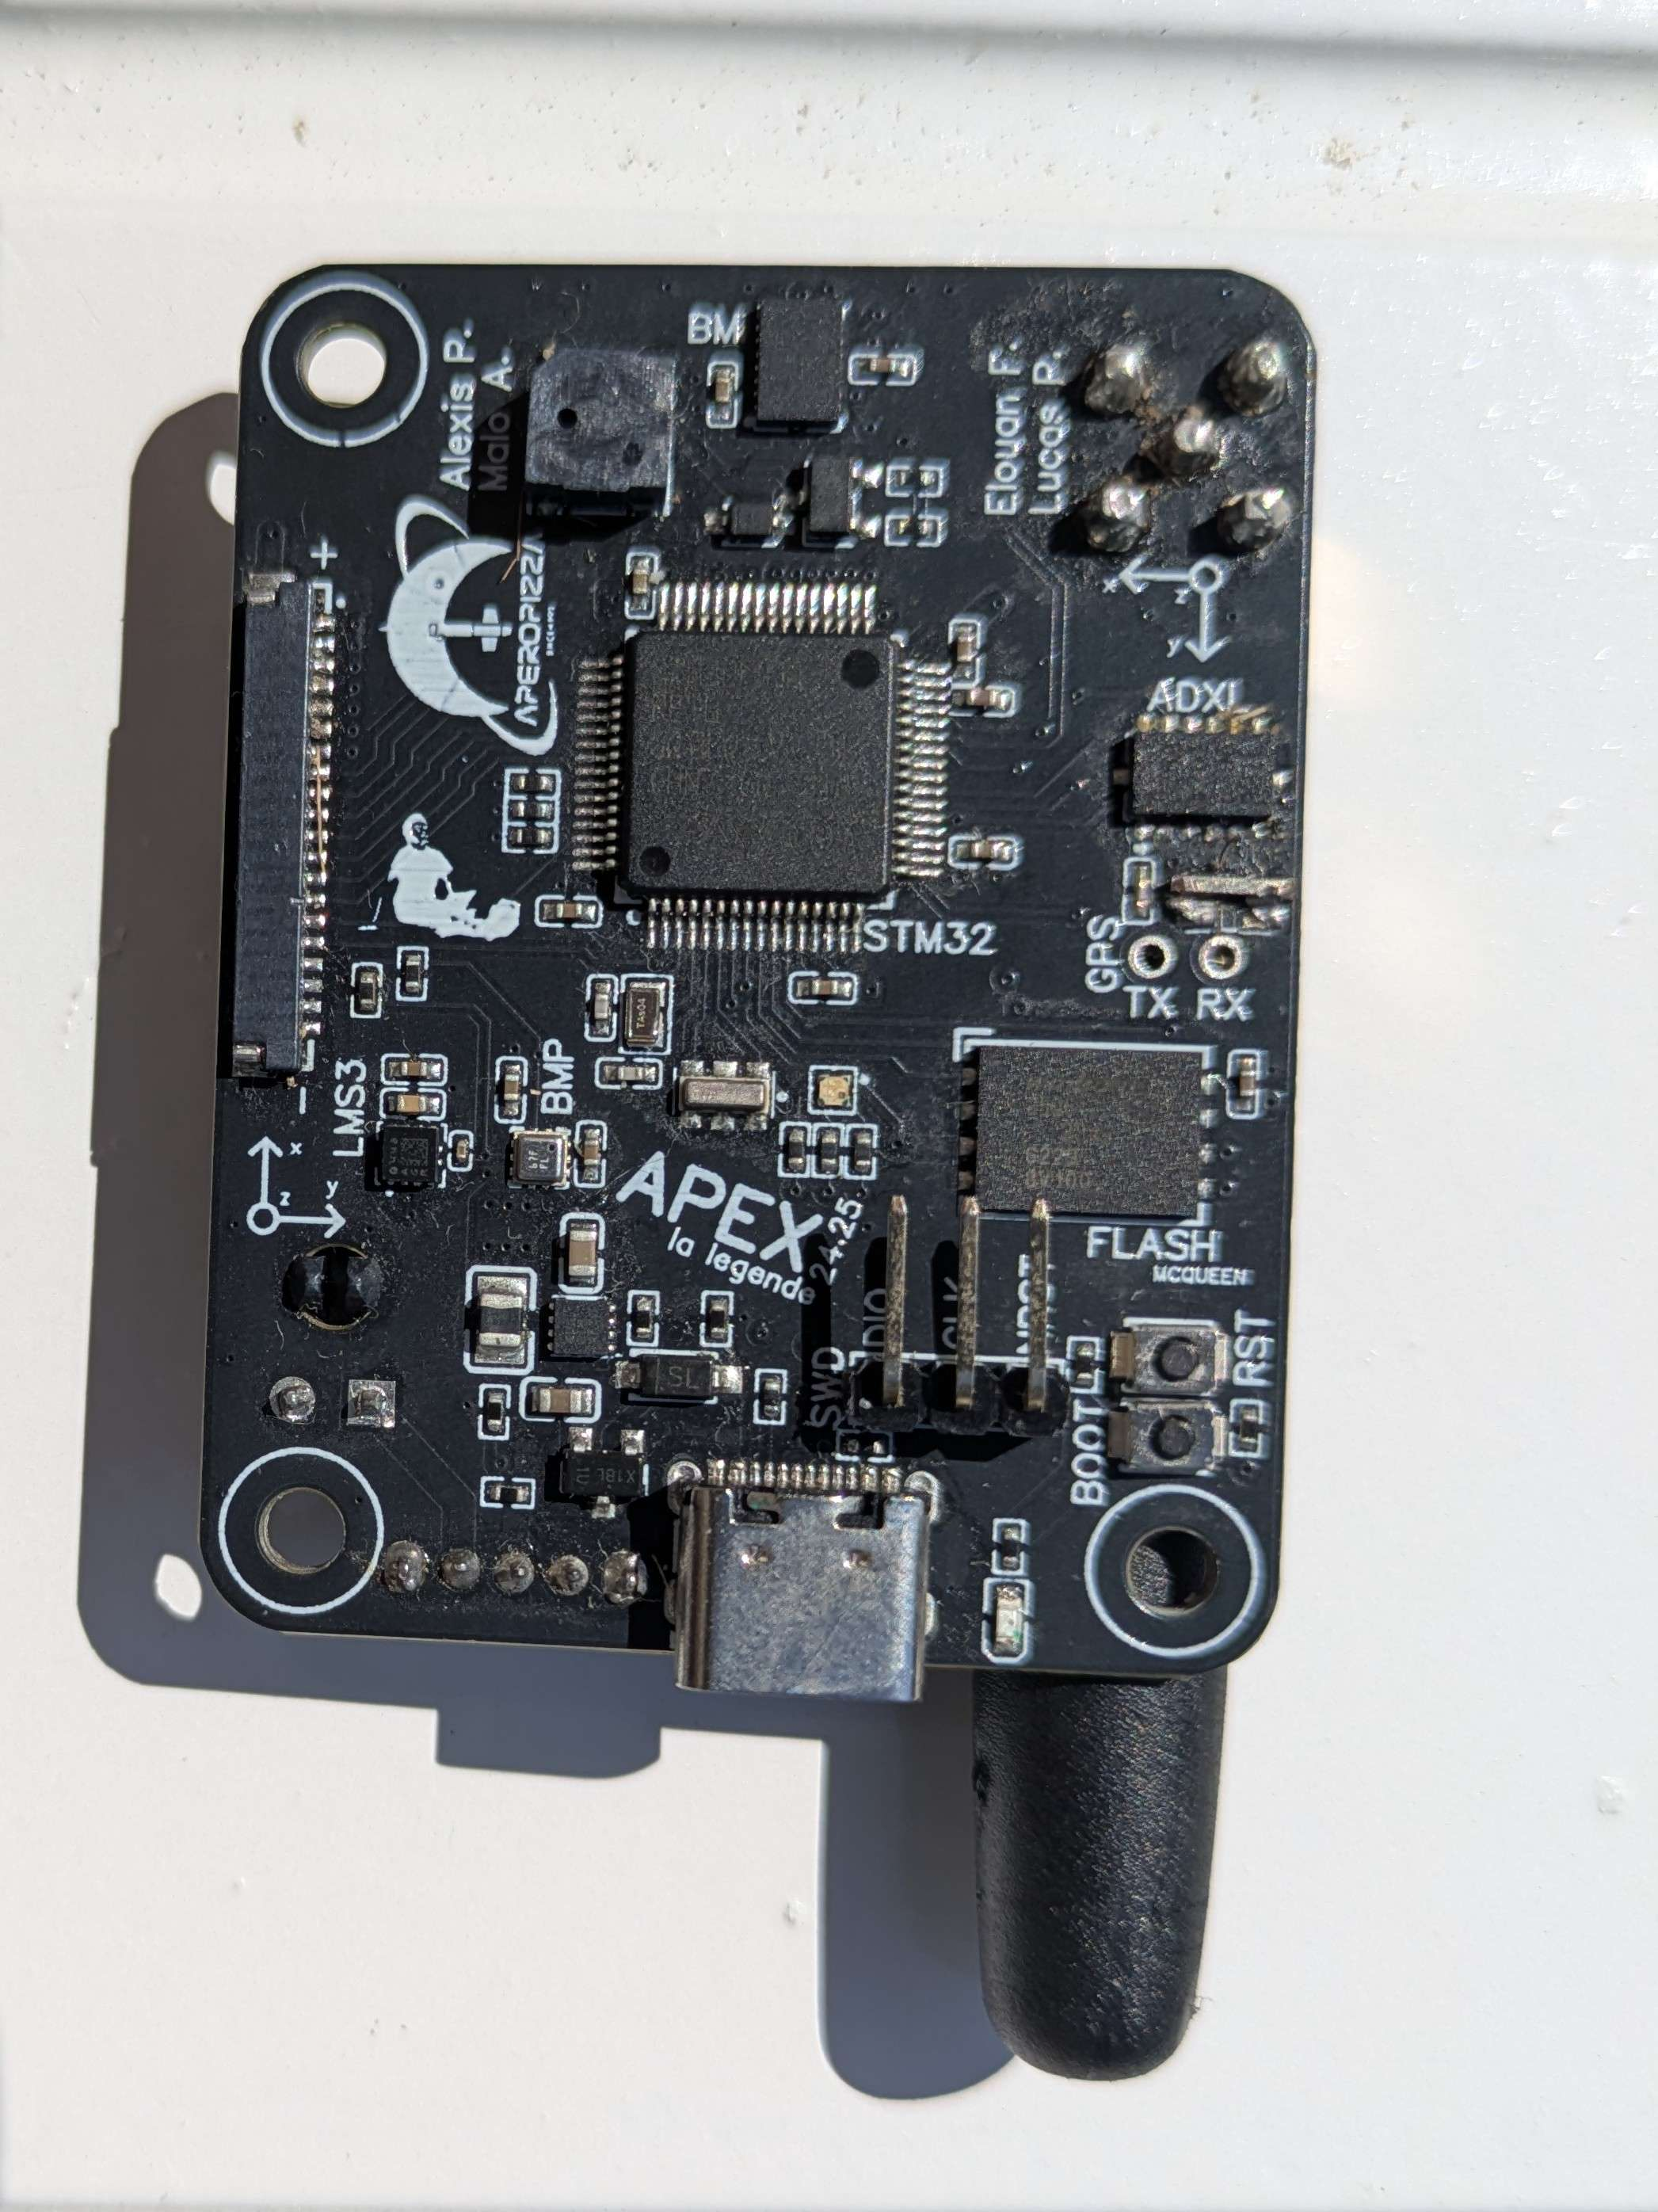
\includegraphics[width=0.7\textwidth]{figures/APEX_FRONT.jpg}
        \caption{face avant}
        \label{fig:apex_front}
    \end{subfigure}
    \caption{Module électronique \gls{APEX}}
\end{figure}
\end{itemize}

Ainsi, SP-02 s’inscrit dans une continuité technique et expérimentale : il hérite des méthodes de conception composite issues
d’Arcturus et SP-01, tout en intégrant la maturité avionique acquise grâce aux projets Unknown et \gls{APEX}. Cette filiation
confère au projet un haut niveau de maturité technologique dès ses premières phases de conception, gage de fiabilité et de
réussite pour la campagne \gls{C'Space} 2026.